\documentclass[12pt]{article}

\usepackage{sbc-template}

\usepackage{graphicx,url}

%\usepackage[brazil]{babel}   
\usepackage[latin1]{inputenc}  

\usepackage{float}

\usepackage{epstopdf}
\usepackage[table]{xcolor}
\usepackage{booktabs}

%\usepackage{caption}
%\usepackage{subcaption}
\newtheorem{myDefinition}{Definition}
     
\sloppy

\title{Radio Communication to Control and Run an Autonomous Mission for UAVs via a Mobile Application}

\author{Thiago R. F. Cavalcante\inst{1,2}, Erickson H. da S. Alves\inst{1,2}, Celso B. Carvalho\inst{2,3} }


\address{Federal University of Amazonas\\
  Av. General Rodrigo Octavio Jord�o Ramos, 1200 - Coroado I, Manaus - AM, Brazil, 69067-005
\nextinstitute
  Master Degree in Electrical Engineering\\
  Federal University of Amazonas, Brazil.
\nextinstitute
  Department of Electronics and Computer\\
  Federal University of Amazonas, Brazil.
  \email{\{thiagorodrigoengcomp, erickson.higor\}@gmail.com, ccarvalho\_@ufam.edu.br}
}

\begin{document} 

\maketitle

\begin{abstract}
  This paper presents the development of an Android application for the industry in order to start the production and supervise the process in production lines. A unmanned aerial vehicle (UAV) is used, equipped with a robotic gripper, which consists in an industrial scenario with an input warehouse, production lines, and a product depot. In the application, there is a mission planner that produces the needed commands for carrying out a given mission (the production of a product), which includes the delivery of inputs brought from the warehouse to the production line until the final product is delivered to the client (product depot). It is presented how the Android application is useful to assist in the supervisioning process for line managers/leaders.
\end{abstract}


\section{Introduction}
% no \IEEEPARstart
\label{sec:introduction}

Logistics has become a competitive and fundamental factor for organizations, involving the management, conservation, and supervision of freight transport. In addition, excellent logistics means customer satisfaction; so speed is still an important factor in a successful logistics process~\cite{drone4logistic}. Currently, one of the solutions to this type of problem is the use of unmanned aerial vehicles (UAVs). Nowadays, UAVs are mostly remotely piloted vehicles (RPV), since their operations are carried out by ground operators. If the tasks performed by a UAV are performed autonomously, it would relieve the work of these operators, since they perform tedious and repetitive tasks~\cite{pascarella2013autonomic}.

One possible improvement of these logistics systems is the increase of the UAVs automation, which results in costs minimization. Consequently, investments and studies related to stand-alone UAVs are important to the smart factories development~\cite{hern2014dhl}. However, one of the main problems for using autonomous UAVs is the system's reliability and intelligence. Thus, increased employment of autonomous UAVs requires the development of devices, which are able to perform tasks and interact with the environment in an intelligent and reliable way.

Autonomous UAVs need to know what will happen in a future instant and what is the best decision to make at the present time; therefore, they require strategies not only to decompose their missions into meaningful sub-tasks, but also to track progress toward mission goals and the evolution of these tasks relative to the autonomous UAVs capabilities~\cite{finn2012developments}. As a consequence, in order to successfully perform a mission, it is recommended to perform task planning~\cite{finn2012developments}. Mission planning problems consist of planning events to meet certain requirements and objectives~\cite{krozel1988search}. Therefore, planning events is one of the main challenges faced in solving this problem.

Both academy and industry have done researches about evaluation and optimization of mission planning in the last years. In \cite{schwarz2012towards} is used ant colony to optimize UAV missions. Another paper investigates energy consumption for a factory and evaluates the logistic planning processes using statistical metrics of evaluation~\cite{muller2012analyzing}.

In this work we present an Android application to supervise production lines in real-time, enabling leaders/managers to check statuses and act on failures. It uses the Drone Kit API, which enables sending commands and receiving updates to/from the drone.

In summary, the main contributions of this study are:
\begin{itemize}
\item an Android app to supervise production lines;
\item methods to control the drone using a smartphone;
\item a mission planner directly implemented in the app.
\end{itemize}
	
\textit{Outline}. Section~\ref{sec:background} provides the fundamentals of mission planning and optimization problems. Section~\ref{sec:uav} describes the UAV movement system used in this work. Section~\ref{sec:method} explains the proposed evaluation methodology in further details. Section~\ref{sec:results} describes the experimental procedures and results in order to explore and demonstrate the potential of methodology, and, finally, Section~\ref{sec:conclusao} concludes this study and describes future work.

%--------------------------------------------
\section{Preliminaries}
\label{sec:background}
%--------------------------------------------

%--------------------------------------------
\subsection{Terminology}
\label{sec:terms}
%--------------------------------------------

Key definitions related to the case study and the application developed in this study need to be clarified. All definitions below are adopted in the remainder of this study.

\begin{myDefinition} 
\textbf{(Mission Command)} 
Mission Command is a command created to execute a task such as to go from one location to another, get a package using a robot gripper, and land a UAV.
\label{def:missioncommand}
\end{myDefinition}

\begin{myDefinition}
\textbf{(Mission)} 
Mission is the set of steps and mission commands that the UAV executes to produce the customer's order.
\label{def:mission}
\end{myDefinition}

\begin{myDefinition}
\textbf{(Warehouse)}
Warehouse is the set of stored raw material available until the moment of entering the productive process. The raw materials, \textit{i.e.}, the inputs available in this work are inputs A, B, and C.
\label{def:almoxarifado}
\end{myDefinition}

\begin{myDefinition} 
\textbf{(Order)}
Order is the requisition of products made by the client. In this study, the products are of type X and Y.
\label{def:pedido}
\end{myDefinition}

\begin{myDefinition}
\textbf{(Production Time)}
Production time is the time required to produce a product X or Y, after making available all the needed inputs for the production, given by the production rule.
\label{def:tempoProducao}
\end{myDefinition}

\begin{myDefinition}
 \textbf{(Production Rule)}
Production rule describes what and how many inputs are needed to produce a particular product.
\label{def:regraProducao}
\end{myDefinition}

\begin{myDefinition}
\textbf{(Mission Planner)}
Mission planner is the agent who performs the planning of a mission, that is, produce all steps and commands needed to carry out a given mission.
\label{def:planejadorMissao}
\end{myDefinition}

\begin{myDefinition}
 \textbf{(Mission File)}
The mission file is a file that is created for the context of this work, with the extension \textsc{.mission} containing the mission itself.
\label{def:arquivoMissao}
\end{myDefinition}

\begin{myDefinition}
 \textbf{(Movement Function)}
The movement function are functions created in Python using the drokekit API to send commands to the UAV by MAVLink protocol.
\label{def:movFunc}
\end{myDefinition}

\begin{myDefinition}
 \textbf{(Production Mission)}
The production mission is the set of steps to produce all the product required by the client.
\label{def:prodMission}
\end{myDefinition}


%--------------------------------------------
%\subsection{DroneKit-Android?s API}
%\label{subsec:dronekit}
%--------------------------------------------

%--------------------------------------------
\subsection{UAV Iris+}
\label{subsec:uaviris}
%--------------------------------------------

The Iris+, introduced by 3DRobotics in Fall 2014, is a 550mm class (measured motor-to-motor) ready-to-fly quadcopter \cite{iris+}. It is powered by a 5100mAh battery driving 4 950kV motors through a 4-in-1 electronic speed controller. It includes a Pixhawk flight control board (described below), an internal uBlox GPS with integrated 3-axis compass for navigation, and a 915MHz radio (or 433MHz, depending on country) for communication with a ground control station. Also included is a full-featured remote control transmitter with a preconfigured receiver onboard the drone. The Iris+ has an advertised flight time of 16-22 min. As of January 2016, the Iris+ retails for \$600, very reasonable for a vehicle with its capabilities.

	\begin{figure}[H]
	\centering
	\includegraphics[width=1.0\columnwidth]{iris.eps}
	\caption{The 3DR Iris+.\label{fig:iris}}
	\end{figure}

Control of the Iris+ is facilitated via the Pixhawk flight control board \cite{meier2011pixhawk}. Developed by researchers at ETH Zurich, the Pixhawk is open source and very widely adopted. It is suitable for use in copters, planes and ground-based rovers. Connectivity options are numerous, allowing for use of a wide array of external devices such as GPS, range finders and companion computers. Internally, the unit integrates a three-axis accelerometer, a three-axis gyroscope, a three-axis compass and a barometer. These sensors allow for determination of motion, orientation, heading and relative altitude, respectively.

    \begin{figure}[H]
	\centering
	\includegraphics[width=0.25\columnwidth]{pixhawk.eps}
	\caption{The Pixhawk flight control board. Numerous ports allow for connection of a multitude of external sensors and devices.\label{fig:pixhawk}}
	\end{figure}

%--------------------------------------------
\subsection{Software}
\label{subsec:software}
%--------------------------------------------
In this section we discuss the third-party open-source software that is integral to the vehicle. It is distinct from that we have developed as part of subsequent research projects. Firmware for the Pixhawk comes in the form of two distinct, but cooperating, open source efforts: APM \cite{ardupilotdev} and PX4 \cite{meieretalPX42015}. Both flight stacks have robust and supportive development communities and are updated frequently. MAVLink \cite{mavilink}, a message-based communication protocol, underlies both efforts. In our vehicles, we use the APM flight stack.

MAVLink provides messages that allow for accessing and changing vehicle parameter values, checking vehicle status and navigation, changing, for example, vehicle position, attitude and velocity. The protocol is extensible, allowing users to define new messages for their purposes. However, the provided message set is sufficiently robust that we have not had the need to do this.

In 2015, 3DR introduced DroneKit-Android, a Android API for developing MAV applications \cite{dronekit}. DroneKit frees researchers and developers from many of the low-level aspects of MAVLink, providing a high-level interface for connecting to, monitoring and controlling a vehicle.

Vehicle configuration and sensor calibration are easily facilitated by ground control station software (GCS). Mission Planner (Windows only) and APM Planner (multi-platform) are both freely available. We use Mission Planner due to its ease of installation.

%%%%%%%%%%%%%%%
\subsection{UAV Movement System}
\label{sec:uav}
%%%%%%%%%%%%%%%

% \subsection{UAV Movement System}

%In this section, we first investigate the UAV platform used (3DR IRIS+) in this study, describing the hardware characteristics and the control framework developed for intralogistics missions. 
The core hardware of the UAV IRIS+ is the Pixhawk and we can control it using a Python library \cite{dronekit}, which uses Micro Air Vehicle Link (MAVLink) protocol~\cite{meier2011pixhawk}. MAVLink is a protocol for communicating with small unmanned vehicle, which is designed as a header-only message marshalling library.

The UAV IRIS+ is integrated into a robot gripper to take and leave packages during missions (cf. Definition~\ref{def:mission}). We have connected a servo motor to the Pixhawk by one of the pulse width modulation (PWM) outputs. Figure~\ref{fig:hardArch} shows the system hardware architecture and the interconnections between each component module. In the hardware architecture shown in the Figure~\ref{fig:hardArch}, we can see the UAV hardware component connections where there is the Pixhawk (flight controller) and its connections between other components such as the compass, GPS, PWM outputs, battery and etc. Moreover, it shows the connection with a robot gripper using a PWM outputs as a signal control for the servo motor in the robot gripper. Finally, it shows the communication between a personal computer (PC) and the UAV via radio control (RC) signal.
%
\begin{figure}[H]
	\centering
	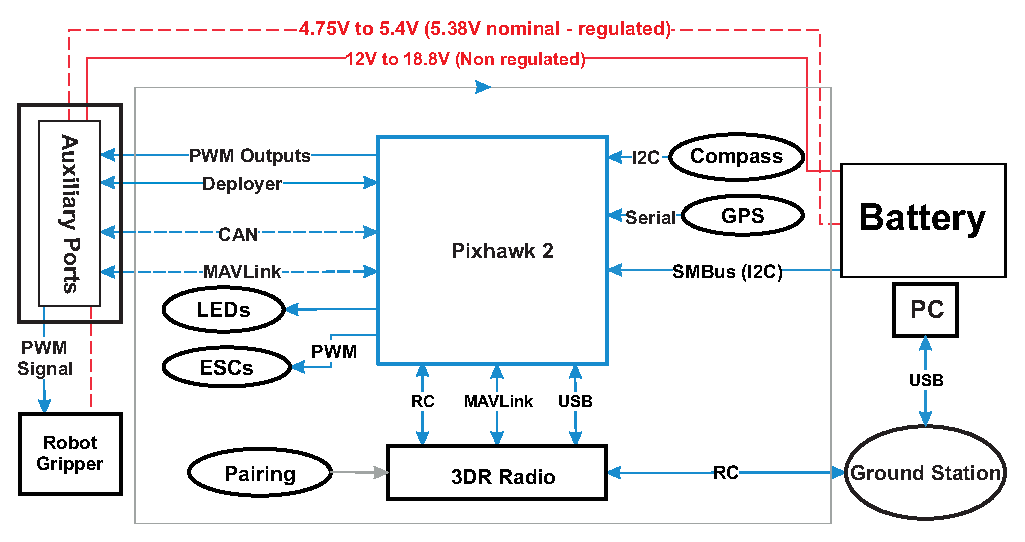
\includegraphics[width=\columnwidth]{arquiteturaIHW.eps}
	\caption{System Hardware Architecture.}
	\label{fig:hardArch}
\end{figure}

In the software architecture, the mission planner (cf. Definition~\ref{def:planejadorMissao}) reads the warehouse inputs and client order and generates the production mission, which contains the list of mission commands needed for producing the required client order. Figure~\ref{fig:sysArch} shows the mission planning framework software components.


In order to control the UAV from a Android application, we have used the dronekit API that translates MAVLink commands to a Java function. The application talks to the UAV using a radio module connected via USB. We have created a bunch of functions in the control program for the most common UAV actions. The movement functions (cf. Definition~\ref{def:movFunc}) are described in Table~\ref{table:movfunc}.
%
%\begin{itemize}
%\item \texttt{TakeOff}: takeoff command of the UAV;
%\item \texttt{GoTo}: command to move the  UAV to a certain location;
%\item \texttt{TakePackage}: command to collect an input/product through a robot gripper;
%\item \texttt{LeavePackage}: command to leave an input or product from a robot gripper;
%\item \texttt{Wait}: command to make a UAV to hover (wait);
%\item \texttt{Land}: command to make a UAV to land.
%\end{itemize}

\begin{table}[H]
\scriptsize
\centering
\resizebox{\textwidth}{!}{
\begin{tabular}{|l|l|}
\hline
\multicolumn{1}{|c|}{\textbf{Command}} & \multicolumn{1}{c|}{\textbf{Description}}           \\ \hline
\texttt{TakeOff}                     & takes off the UAV                                   \\ \hline
\texttt{GoTo}                        & moves the UAV to a certain location                 \\ \hline
\texttt{TakePackage}                 & takes an input/product (gripper) \\ \hline
\texttt{LeavePackage}                & leaves an input/product (gripper)   \\ \hline
\texttt{Wait}                        & makes the UAV to hover (wait)                       \\ \hline
\texttt{Land}                        & lands the UAV                                       \\ \hline
\end{tabular}}
\caption{Description of movement functions}
\label{table:movfunc}
\end{table}


\begin{figure}[H]
	\centering
	\includegraphics[width=\columnwidth]{sysArch.eps}
	\caption{System's Architecture.\label{fig:sysArch}}
\end{figure}


%\subsection{Mission Planning}
%\label{mission}


%%%%%%%%%%%%%%%
\section{Methodology}
\label{sec:method}
%%%%%%%%%%%%%%%

%\commentib{Modifique o t\'itulo (expanda). Metodologia de qu\^e?? Tente fazer algo parecido com o do trabalho.}

%In this section, we evaluate the algorithm mission cost and describe a case study to a UAV and contents about mission planning.

%%%%%%%%%%%%%%%%%%%%%%%%%%%%%%%%%%%%%
\subsection{Case Study: UAV Intralogistics Mission}
\label{sec:ec}
%%%%%%%%%%%%%%%%%%%%%%%%%%%%%%%%%%%%%

In order to model the mission planning problem as an optimization problem, the case study shown in Figure~\ref{fig:useCase} is used.
%
\begin{figure}[ht]
	\centering
	\includegraphics[width=0.85\columnwidth]{useCase.eps}
	\caption{Case Study Representation.\label{fig:useCase}}
\end{figure}
	
Figure~\ref{fig:useCase} shows that there are three types of inputs in the warehouse (\textit{i.e.}, A, B, and C) and two production lines that produce two different products (\textit{i.e.}, X and Y). Each production line produces only one type of product and has a characteristic production time (cf. Definition~\ref{def:tempoProducao}). Figure~\ref{fig:useCase} shows that to produce a product of type X, two inputs of type A and one input of type C are required, and to produce a product of type Y, two inputs of type B and one input of type C are required. The production time of a X product is $4 p.u.$ and the time of production of product Y is $6 p.u.$. A production unit ($1 p.u.$) is considered to be a \texttt{GoTo} command performed by the UAV.

The task to be performed is the production of the client order (cf. Definition~\ref{def:pedido}), where a given UAV collects supplies from the warehouse, takes that to the production line, and once the production of a certain product is finished, the UAV delivers it to the client.

\subsection{UAV Controller App}
\label{subsec:app}

We developed an Android application to connect to the UAV via usb (radio signal module) or udp (simulated uav) in order to create a client order and make the UAV executes it autonomously and the user can visualize and supervise the operation.

\begin{figure}[H]
\centering
\begin{minipage}{.55\textwidth}
  \centering
  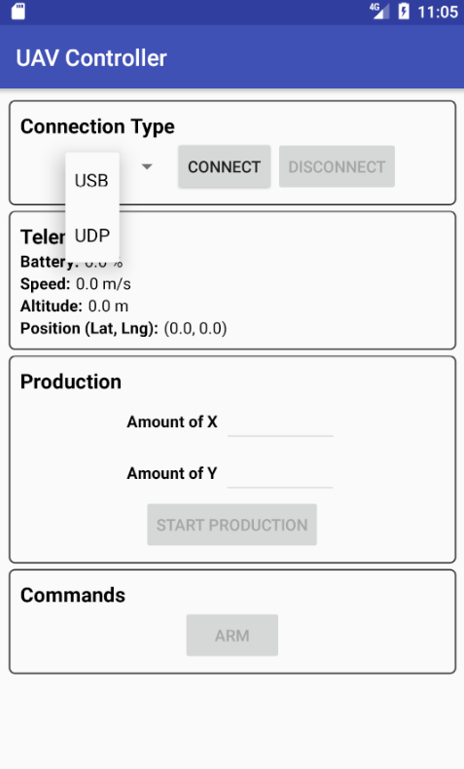
\includegraphics[width=.7\linewidth]{appMain}
  \captionof{figure}{Main Screen.}
  \label{fig:appMain}
\end{minipage}%
\begin{minipage}{.55\textwidth}
  \centering
  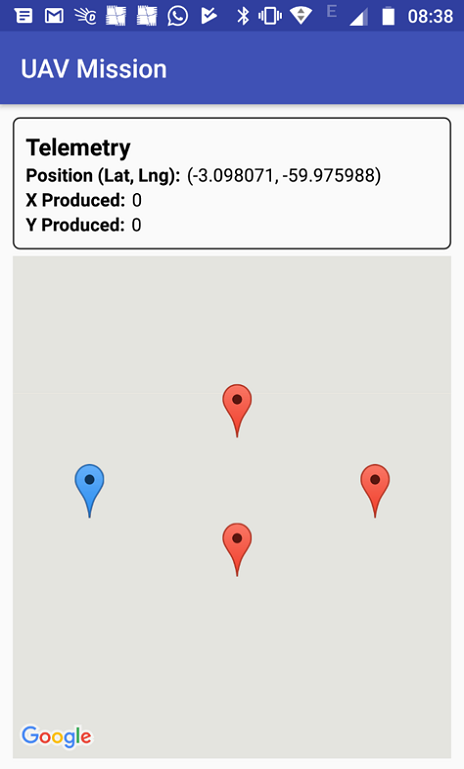
\includegraphics[width=.7\linewidth]{appSec}
  \captionof{figure}{Secondary Screen.}
  \label{fig:appSec}
\end{minipage}
\end{figure}

Internally in the app, it's implemented the mission planner (cf. Definition~\ref{def:planejadorMissao}) and the controller module to send commands to the UAV via radio using the MAVLink protocol in the dronekit API.

\subsubsection{App Mission Planner}
\label{subsubsec:mp}
In the Mission Planner strategy, the UAV starts to bring all the necessary inputs to make the first product X, taking all the A, B and C inputs, respectively, to the production line X. After bring all the necessary inputs to produce the first X product, the production line X starts to produce the X product and while the production line X is producing, the UAV goes to the warehouse to get the necessary inputs to produce the next product (the planner produce firstly the X products e then all the Y products). However, when the X product finishes producing, the UAV knows the instant and goes to the production line to get the X product to bring to the client place; and after that, the UAV goes back to bring the rest of the inputs. The UAV keeps work in the same way until it brings all the products to the client place.

%%%%%%%%%%%%%%%%%%%%%%%%%%%%%%%%%%%%%
\section{Experimental Evaluation}
\label{sec:results}
%%%%%%%%%%%%%%%%%%%%%%%%%%%%%%%%%%%%%
In this section we can see the experimental results of the Android application to control a UAV as described in Section~\ref{sec:ec}.

The Table~\ref{table:tests} shows the experiments tested in a real UAV and a virtual UAV, in order to compare the results in both environments. As we can see, when the virtual UAV is used, the mission gets a smaller flight time than in the real UAV. That is because the radio communication used in the real drone is affected by noises in the environment.
\begin{table}[H]
\centering
\resizebox{\textwidth}{!}{
\begin{tabular}{@{}ccc@{}}
\cmidrule(l){2-3}
                                        & \cellcolor[HTML]{FF7774}\textbf{Real UAV} & \cellcolor[HTML]{5FCE89}\textbf{Virtual UAV} \\ \cmidrule(l){2-3} 
\cellcolor[HTML]{C0C0C0}\textbf{Tests} & \textit{\textbf{Flight Time (s)}}            & \textit{\textbf{Flight Time (s)}}            \\
\cellcolor[HTML]{C0C0C0}1               & 441,72                                       & 430,830                                       \\
\cellcolor[HTML]{C0C0C0}2               & 440,18                                       & 436,885                                       \\
\cellcolor[HTML]{C0C0C0}3               & 447,51                                       & 441,681                                       \\
\cellcolor[HTML]{C0C0C0}4               & 438,19                                       & 441,277                                       \\
\cellcolor[HTML]{C0C0C0}5               & 445,85                                       & 451,865                                       \\ \bottomrule
\end{tabular}}
\caption{Mission Flight Time Tested in Real and Virtual UAV.\label{table:tests}}
\end{table}


\section{Conclusion}
\label{sec:conclusao}
%---------------------------------

We have presented an evaluation methodology for UAV mission planner in an industrial production scenario, as described in Section~\ref{sec:method}. We have developed an Android application to supervise production status and allow real-time monitoring for line managers/leaders.
 
In addition, we have developed a framework for mission planning, command and control for intralogistics mission using a commercial UAV. We used an UAV to solve intralogistics problems using the dronekit API to control and command adopting a high-level programming language.

Future work includes the use of computational vision for the recognition of inputs, and improvements of the optimization problem modeling for better results in cost evaluation. Supplementary, we will make experiments in a cooperative work environment where the number of UAVs is greater than two. In order to improve our results, we will develop more planner strategies such as an algorithm that produces different types of products simultaneously. Moreover, we will evaluate the communication between the drone and the application using different frameworks/protocols, in order to improve the supervision step.

\bibliographystyle{sbc}
\bibliography{sbc-template}

\end{document}
